% % % % % % % % % % % % % % % % % % % % % % % % % % % % % % % % % % % % % % % % % % % %
%                                                                                     %
% Short Sectioned Assignment LaTeX Template Version 1.0 (5/5/12)                      %
% This template has been downloaded from: http://www.LaTeXTemplates.com               %
%                                                                                     %
% Original author:  Frits Wenneker (http://www.howtotex.com)                          %
%                                                                                     %
% Modified by: Fco Javier Sueza Rodríguez (fcosueza@disroot.org)                      %
%                                                                                     %
% Changes:                                                                            %
%	    - Custom Chapters, Sections and Subsections (titlesec package)                %
%           - Document type scrbook (oneside)                                         %
%           - Use babel-lang-spanish package and marvosym                             %
%           - Use hyperref, enumitem, tcolorbox and glossaries packages               %
%           - Use Time New Roman (mathptmx), Helvetic and Courier fonts               %
%                                                                                     %
% License: CC BY-NC-SA 3.0 (http://creativecommons.org/licenses/by-nc-sa/3.0/)        %
%                                                                                     %
% % % % % % % % % % % % % % % % % % % % % % % % % % % % % % % % % % % % % % % % % % % %

%-----------------------------------------------%
%	              Packages                  %
%-----------------------------------------------%

\documentclass[paper=a4, fontsize=11pt, oneside]{scrbook}

% ---- Text Input/Output ----- %

\usepackage[T1]{fontenc}
\usepackage[utf8]{inputenc}
\usepackage{mathptmx}
\usepackage[scaled=.92]{helvet}
\usepackage{courier}
\usepackage[indent=12pt]{parskip}

\usepackage{geometry}
\geometry{verbose,tmargin=3cm,bmargin=3cm,lmargin=2.6cm,rmargin=2.6cm}

% ---- Language ----- %

\usepackage[spanish]{babel}
\usepackage{marvosym}

% ---- Another packages ---- %

\usepackage{amsmath,amsfonts,amsthm}
\usepackage{graphics,graphicx}
\usepackage{titlesec}
\usepackage{fancyhdr}
\usepackage{tcolorbox}
\usepackage{hyperref}
\usepackage{enumitem}
\usepackage[automake]{glossaries}

%--------------------------------------------------------------------%
%                      Customizing Document                          %
%--------------------------------------------------------------------%


% ----------- Custom Chapters, Sections and Subsections -------------- %

\titleformat{\chapter}[display]
			{\bfseries\Huge}
			{Tema \ \thechapter} {0.5ex}
			{\vspace{1ex}\centering}

\titleformat{\section}[hang]
			{\bfseries\Large}
			{\thesection}{0.5em}{}

\titleformat{\subsection}[hang]
			{\bfseries\large}
			{\thesubsection}{0.5em}{}

\titleformat{\subsubsection}[hang]
			{\bfseries\large}
			{\thesubsubsection}{0.5em}{}

\hypersetup{
    colorlinks=true,
    linkcolor=black,
    urlcolor=magenta
}

% ------------------- Custom heaaders and footers ------------------- %

\pagestyle{fancyplain}

\fancyhead[]{}
\fancyfoot[L]{}
\fancyfoot[C]{}
\fancyfoot[R]{\thepage}

\renewcommand{\headrulewidth}{0pt} % Remove header underlines
\renewcommand{\footrulewidth}{0pt} % Remove footer underlines

\setlength{\headheight}{13.6pt} % Customize the height of the header

% --------- Numbering equations, figures and tables ----------------- %

\numberwithin{equation}{section} % Number equations within sections
\numberwithin{figure}{section} % Number figures within sections
\numberwithin{table}{section} % Number tables within sections

% ------------------------ New Commands ----------------------------- %

\newcommand{\horrule}[1]{\rule{\linewidth}{#1}} % Create horizontal rule command


%----------------------------------------------------------------------------------------
%	TÍTULO Y DATOS DEL ALUMNO
%----------------------------------------------------------------------------------------

\title{
\vspace{10ex}
\normalfont \normalsize
\Huge \textbf{Tarea 6: Programación de Bases de Datos}
}
\author{Francisco Javier Sueza Rodríguez}
\date{\normalsize\today}

%----------------------------------------------------------------------------------------
%                                     DOCUMENTO
%----------------------------------------------------------------------------------------
\begin{document}

\maketitle

\thispagestyle{empty}

\vspace{62ex}

\begin{center}
    \begin{tabular}{l l}
        \textbf{Centro}: & IES Aguadulce \\
        \textbf{Ciclo Formativo}: & Desarrollo Aplicaciones Web (Distancia)\\
        \textbf{Asignatura}: & Bases de Datos\\
        \textbf{Tema}: & Tema 6 - Programación de Bases de Datos\\
    \end{tabular}
\end{center}

\newpage

\section{Caso Práctico}
Siguiendo con los casos prácticos de las unidades anteriores, el equipo de Ana ya sabe realizar  todo tipo de consultas y todo tipo de  operaciones como la inserción, eliminación y la actualización de datos. Ahora de lo que se trata de es de aumentar las posibilidades que nos ofrecen las bases de datos aprendiendo a realizar pequeñas aplicaciones como procedimientos, funciones y triggers.

Para ello, se han reunido para ver cómo van a abordar esta tarea y han decidido realizar esta aplicaciones en el SGBD Oracle Database Express Edition 11g Release 2 y el  lenguaje de programación PL SQL. Para ello también van a instalar SQL Developer que les permitirá conectarse a una BD de Oracle y cuya interafaz gráfica es mucho más amigable y potente para desarrollar que la que proporciona el propio Oracle Express Edition.

\section{Actividades}

\subsection{Enunciado}
Para automatizar ciertas operaciones en la BD y que puedan ser llamadas desde otras aplicaciones se desea programar algunas funcionalidades en la base de datos \textbf{CUIDATUCUERPO} y tienes que implementar dos procedimientos, una función y un disparador.

\begin{enumerate}[label=\Alph*)]
    \item Crear un procedimiento que reciba como parámetro el número de fisioterapeuta  y muestre por pantalla un listado con todos los clientes que han tenido una cita con él. Debe mostrar el nombre y apellidos de los distintos clientes, así como el DNI, teléfono, fecha\_hora  y el precio de la cita ordenados por fecha\_hora de menor a mayor. Por último en la última línea debe aparecer el precio total de las citas.  Puedes guiarte con la siguiente salida por pantalla:

    \begin{figure}[H]
        \centering
        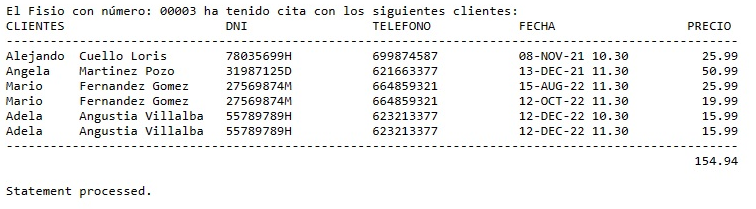
\includegraphics[scale=0.70]{formato-salida.png}
        \caption{Formato de Salida del Procedimiento del Apartado A}
    \end{figure}

    \begin{itemize}
        \item Para formatear la salida en cada una de las líneas se utiliza la función DMBS\_OUTPUT.PUT\_LINE que imprime en cada línea la información que se pasa como parámetros concatenando si es necesario varios valores o literales.
        \item Para proporcionar espacios en blanco a la derecha o a la izquierda se puede utilizar las funciones RPAD y LPAD respectivamente. Puedes encontrar más información en los contenidos de la unidad 4 de este módulo donde se explican estas funciones en el apartado 5.2. Funciones de cadena de caracteres para Oracle.
    \end{itemize}

    \item Crear un procedimiento que reciba como parámetro el DNI de un cliente. El procedimiento debe calcular la cantidad de citas de fisioterapia que ha tenido y el precio total bruto de esas citas. También en función del porcentaje de descuento que tiene ese cliente el procedimiento debe calcular el descuento, y  el precio total de las citas con el descuento aplicado.

    El procedimiento debe mostrar por pantalla el dni del cliente, nombre, apellidos, número de citas, precio total bruto (sin descuento), descuento, precio total neto  (con descuento). Puedes guiarte con la siguiente salida por pantalla:

   \begin{figure}[H]
        \centering
        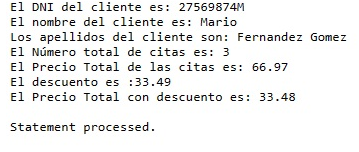
\includegraphics[scale=0.80]{formato-salida-B.png}
        \caption{Formato Salidad del Procedimiento del Apartado B}
    \end{figure}

    \item Crea una función que reciba el nombre de un sala  y nos indique el número de profesores de pilates que dan clase en esa sala.

    \item Crear un disparador (trigger) que se dispare cada vez que se realice la venta de un producto de manera que se disminuya el stock del producto  en la cantidad vendida. En este caso se deberá comprobar el funcionamiento del trigger, para ello deberás insertar algunos registros en la tabla VENDEN y posteriormente consultar la tabla PRODUCTOS para comprobar que se ha actualizado el campo Stock.
\end{enumerate}

\subsection{Solución}
En esta tarea vamos a programar diferentes procedimientos, funciones y disparadores que nos ayudarán a automatizar ciertas tareas de nuestra base de datos, usando para ello el lenguaje \textbf{PL/SQL}.

\begin{enumerate}[label=\Alph*)]
    \item \textbf{Procedimiento NumeroClientesFisio}:

    Este procedimiento se va a encargar de, dado un \textbf{número de fisioterapeuta}, mostrar \textbf{todos los clientes} que han tenido cita con el, mostrándolos en una tabla. A continuación se muestra una captura del procedimiento correctamente creado en Oracle XE.

    \begin{figure}[H]
        \centering
        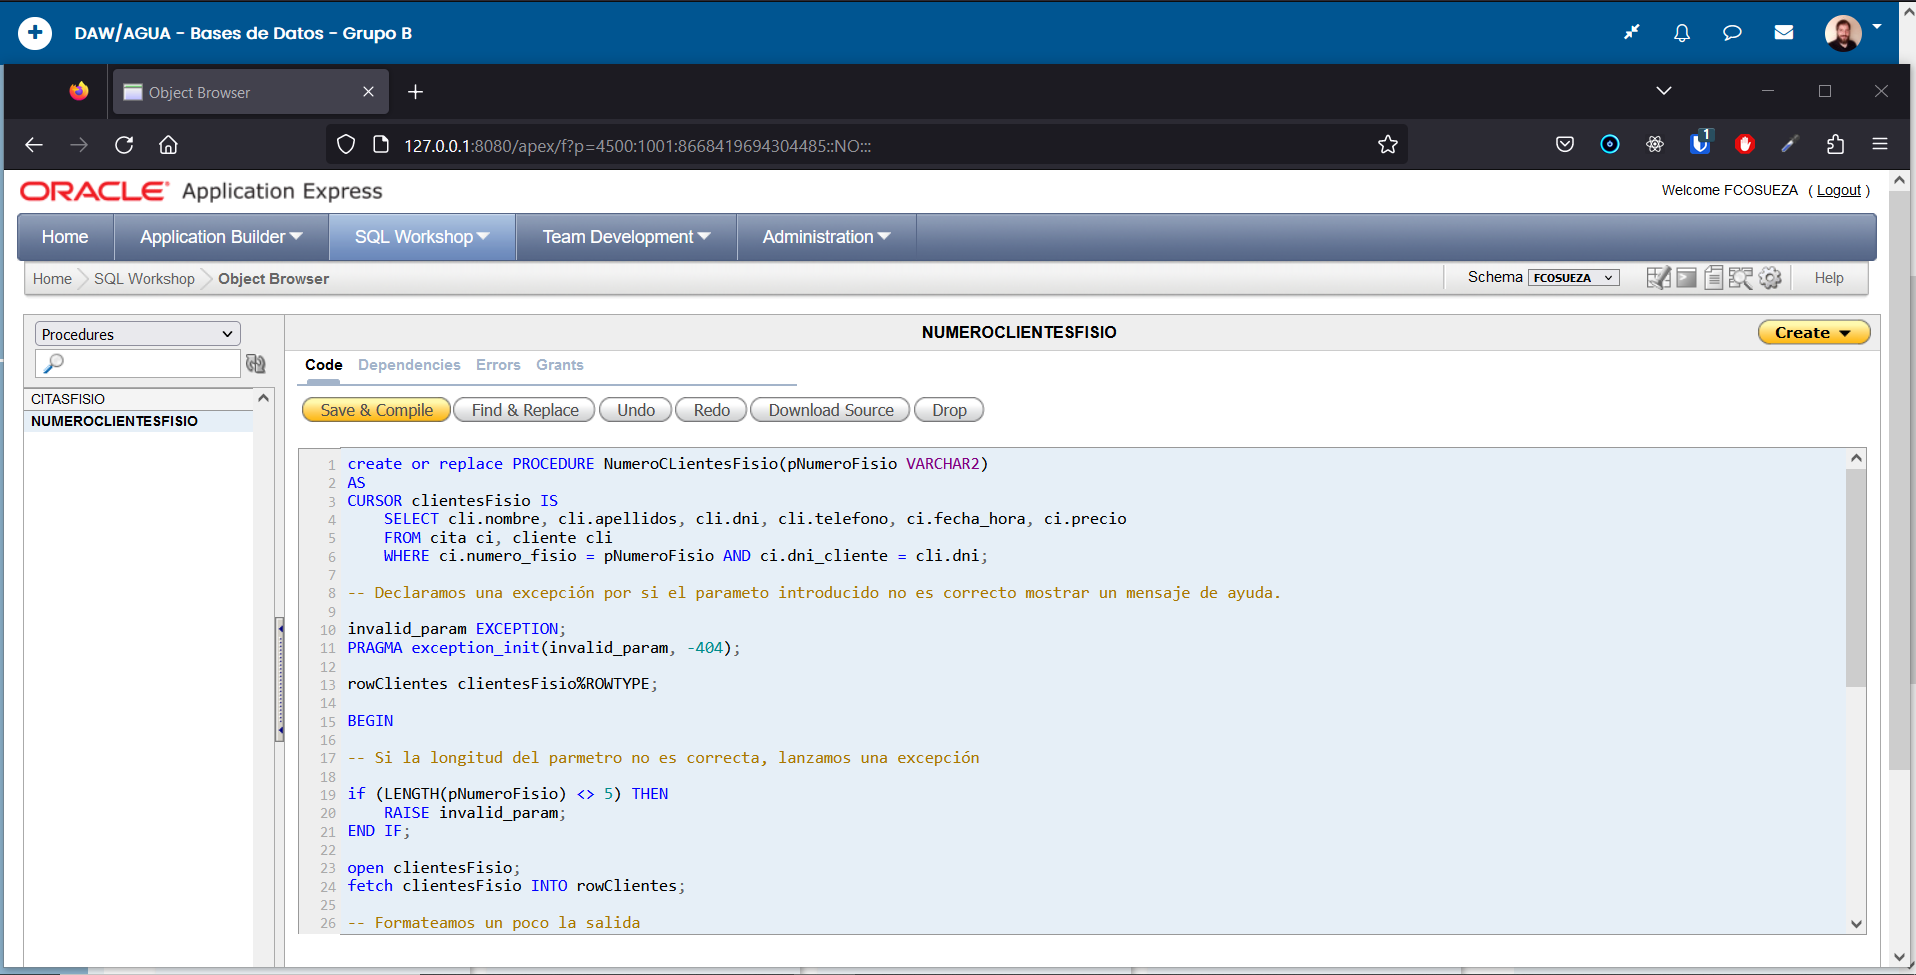
\includegraphics[scale=0.33]{procedimiento-1-creado.png}
        \caption{Procedimiento NumeroClientesFisio creado en Oracle XE}
    \end{figure}

    Hemos creado \textbf{un procedimiento} que acepta como \textbf{parámetro} el \textbf{número de un fisioterapeuta}. Con este número, realizamos \textbf{una consulta} donde vamos a obtener todos los clientes que han tenido cita con el y los datos de estos.

    Para ir \textbf{procesando} esta información se ha creado un \textbf{cursos explícito}, donde vamos ir almacenando las diferentes filas del resultado de la consulta, y una variable de tipo \textbf{\%ROWTYPE} donde vamos ir almacenando los resultados del cursor.

    Por último, se ha mostrado la salida con \textbf{DBMS\_OUTPUT}, formateándola para que se muestre en una tabla, haciendo uso intensivo de la función \textbf{RPAD} y la función \textbf{TO\_CHAR} para formatear la salida de la fecha.

    \begin{figure}[H]
        \centering
        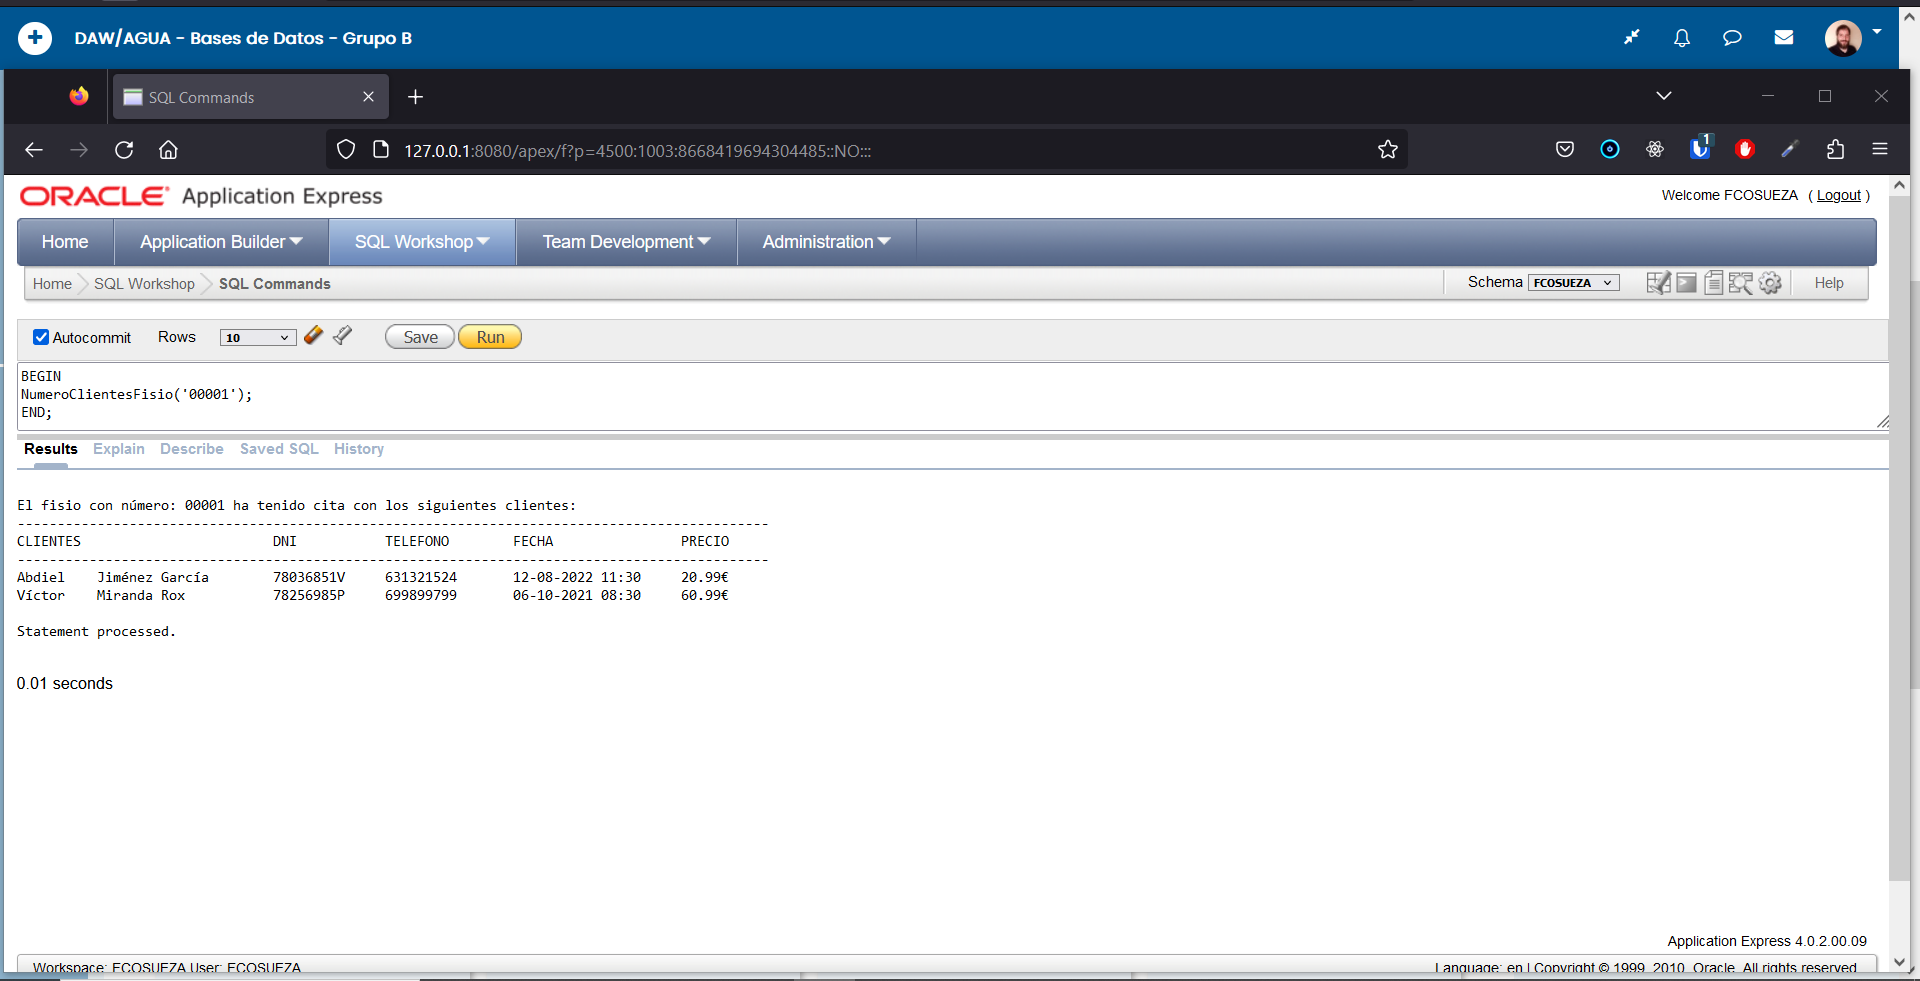
\includegraphics[scale=0.30]{procedimiento-1-ejecucion.png}
        \caption{Ejecución de NumeroClientesFisio en Oracle XE}
    \end{figure}

    \item \textbf{Procedimiento CitasFisio}:

    El segundo procedimiento que hemos creado es \textbf{CitasFisio}, el cual se encarga de mostrar todas las citas que ha tenido un cliente con fisioterapeutas, mostrando el nombre y apellidos del cliente, DNI, el número total de citas, el precio total de las citas y más datos.

    En este caso, se ha optado por \textbf{no usar} las funciones \textbf{COUNT} y \textbf{SUM} para realizar los cálculos en la consulta a la base de datos, sino que hemos usado \textbf{PL/SQL} para realizar estos cálculos.

    En primer lugar, el procedimiento recibe como \textbf{parámetro} el \textbf{DNI de un cliente}. Con este DNI, hacemos una \textbf{consulta} en las tablas \textbf{cita} y \textbf{clientes} para comprobar cuantas citas hay con ese DNI, obteniendo de paso todos los datos necesarios.

    Al igual que en el ejemplo anterior, hemos creado un \textbf{cursos explícito} para ir iterando por las filas del resultado de la consulta. El \textbf{número de filas} que tenga el resultado, coincide con el \textbf{número de citas} que ha tenido un cliente, por lo que cuando hemos llegado al final del resultado, la opción \textbf{\%ROWCOUNT} del cursor nos devolverá el número exacto de citas que hay con ese DNI, es decir, el número de filas. Por lo que hemos \textbf{iterado} sobre el \textbf{cursor}, aprovechando para acumular el \textbf{precio de cada cita} en una variable, obteniendo así el total bruto del coste de las citas.

    Tras esto, se ha \textbf{calculado el descuento} que supone sobre ese total, que depende del descuento que tenga asignado el cliente, y se ha almacenado dicha cantidad en una variable.´

    A continuación se han mostrado los datos usando \textbf{DBMS\_OUTPUT}.

    También comentar que hemos \textbf{creado una excepción} para mostrar una mensaje en caso de que el DNI no tenga la longitud correcta.

    En la siguiente captura podemos ver como se ha creado correctamente el procedimiento.

    \begin{figure}[H]
        \centering
        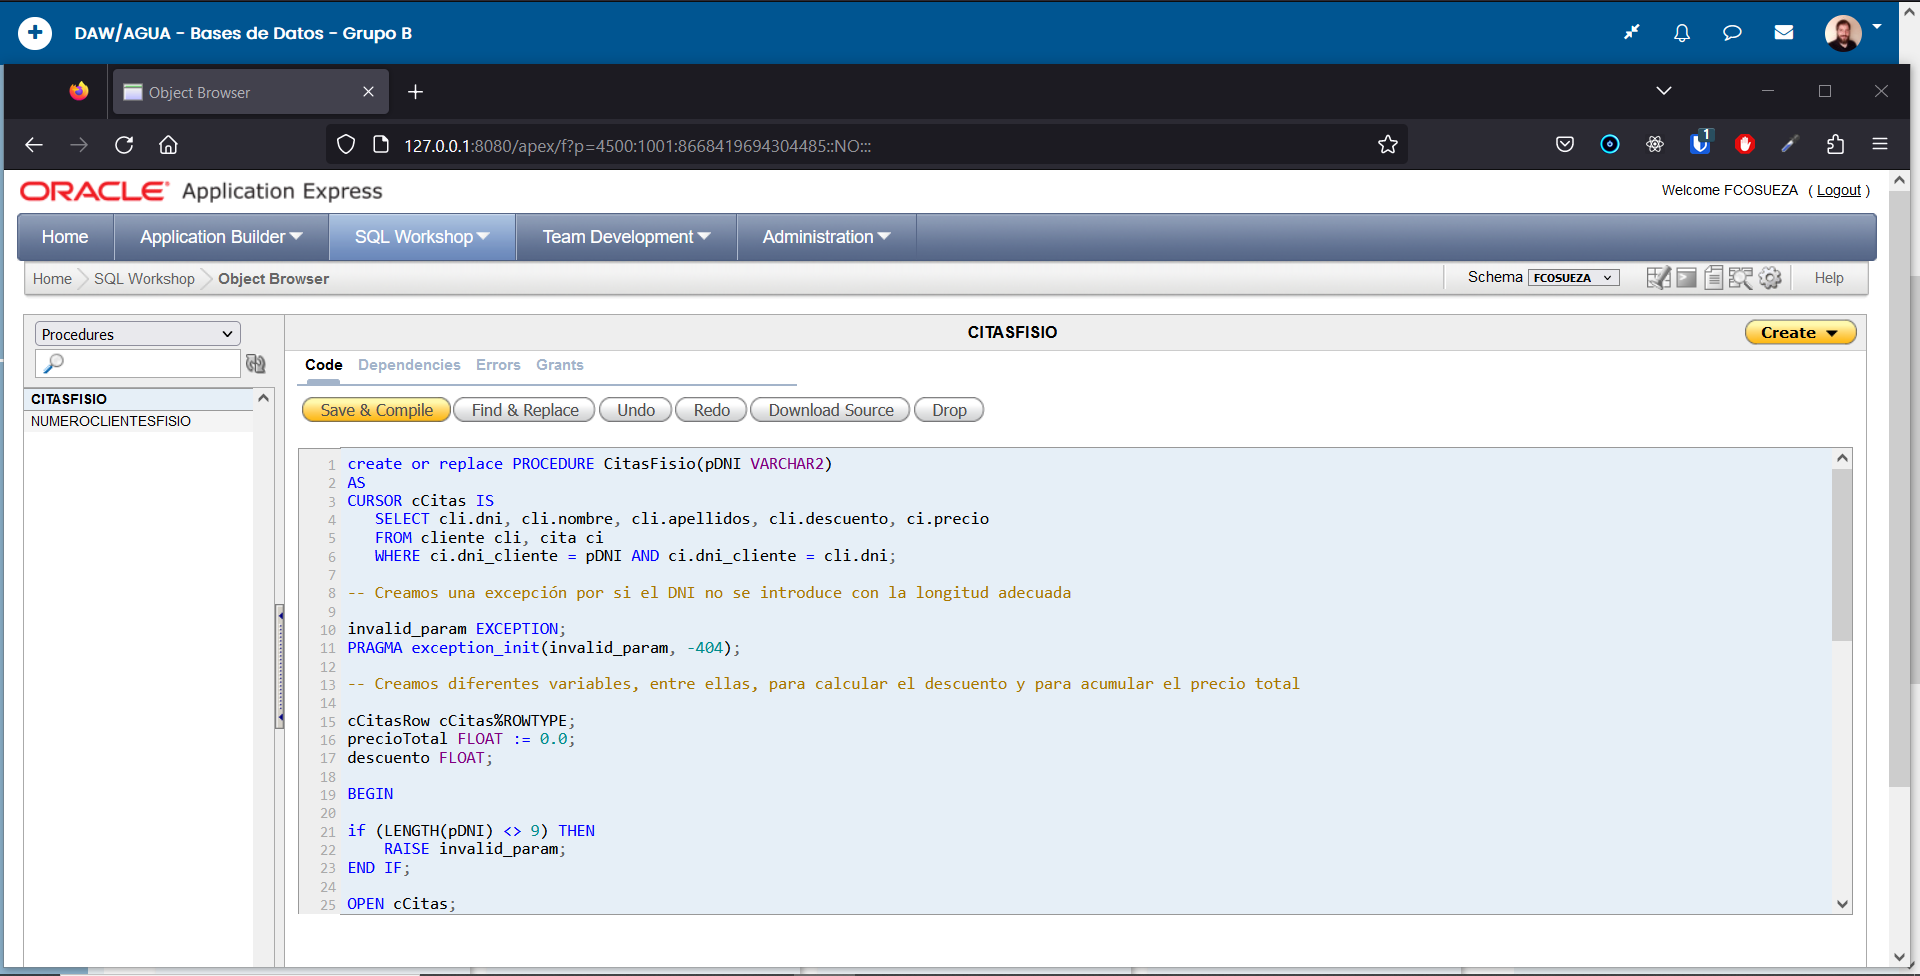
\includegraphics[scale=0.33]{procedimiento-2-creado.png}
        \caption{Procedimiento CitasFisio creado en Oracle XE}
    \end{figure}

    Tras la creación, lo hemos ejecutado dentro de una cláusula \textbf{BEGIN} para comprobar que funcionaba correctamente, ofreciendo el resultado que esperábamos como vemos en la siguiente figura.

    \begin{figure}[H]
        \centering
        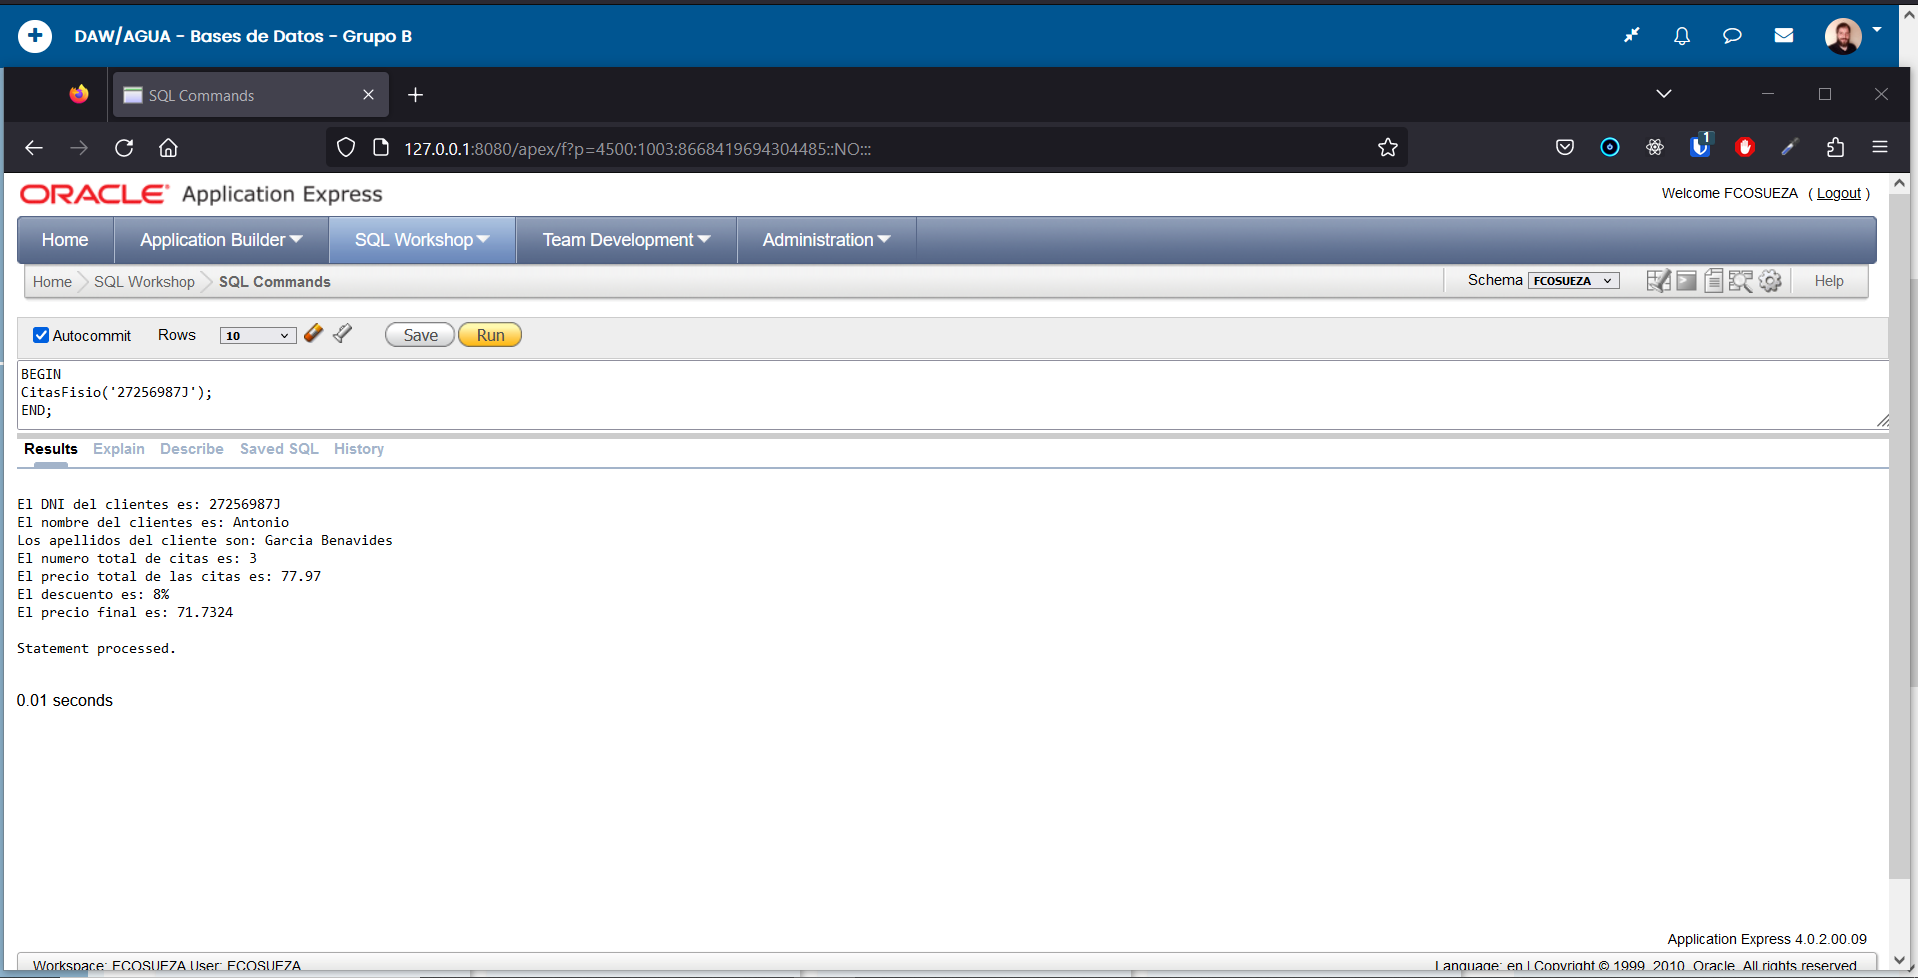
\includegraphics[scale=0.33]{procedimiento-2-ejecucion.png}
        \caption{Procedimiento CistasFisio ejecutado en Oracle XE}
    \end{figure}

    \item \textbf{Función NumeroProfesoresSala}:

    En este caso no se ha creado un procedimiento, sino una \textbf{función}. Esta función recibe como \textbf{parámetro} un código de sale y devuelve el \textbf{número de profesores diferentes} que imparten clases en ella.

    Para implementar, hemos creado una \textbf{variable}, llamada \textbf{nProfesores} en la definición de la función. Con el código de sala, solo hemos tenido que realizar una consulta, usando la función \textbf{COUNT} junto con \textbf{DISTINC} lo que nos devuelve el número de profesores diferentes que dan clases en dicha sala. Esta información, se ha almacenado en la variable \textbf{nProfesores} y se ha devuelto por la función.

    En la siguiente captura se puede ver la función creada.

    \begin{figure}[H]
        \centering
        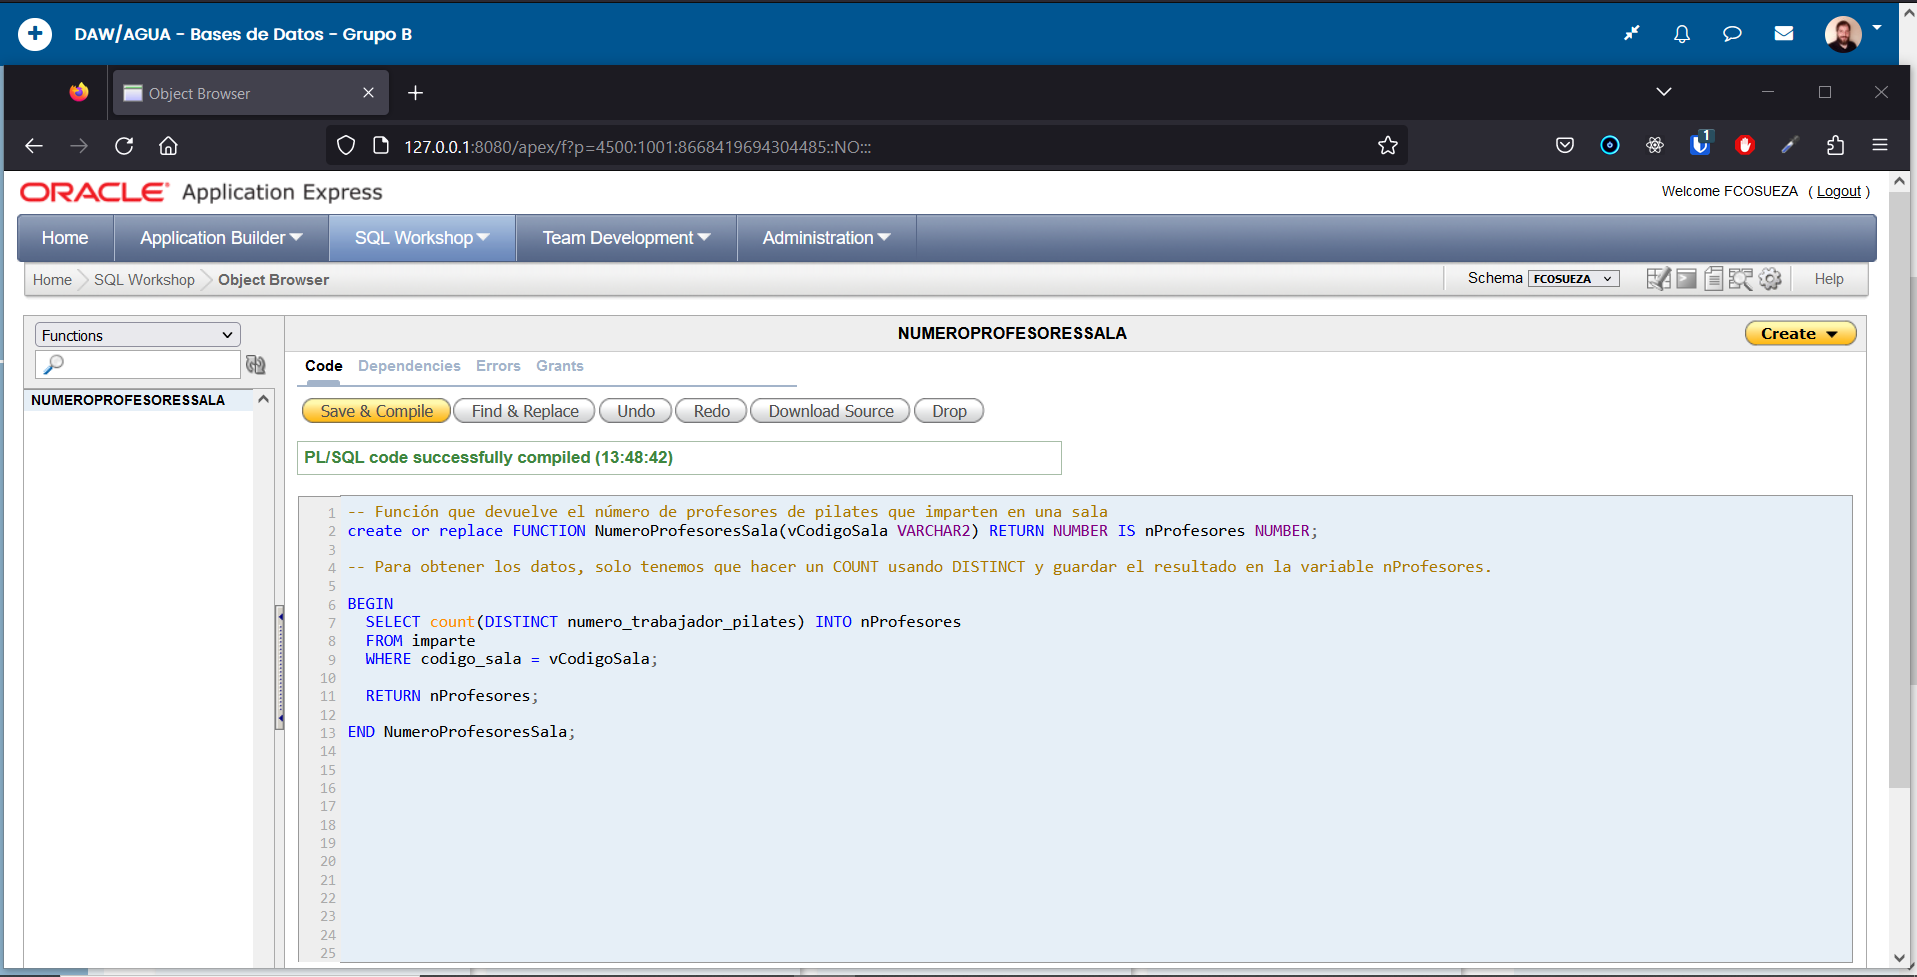
\includegraphics[scale=0.33]{funcion-creada.png}
        \caption{Función NumeroProfesoresSala creada en Oracle XE}
    \end{figure}

    Tras crearla, hemos probado su funcionamiento introduciendo la función dentro de un \textbf{DBMS\_OUTPUT} para comprobar que muestra los datos correctamente, como vemos en la siguiente captura.

    \begin{figure}[H]
        \centering
        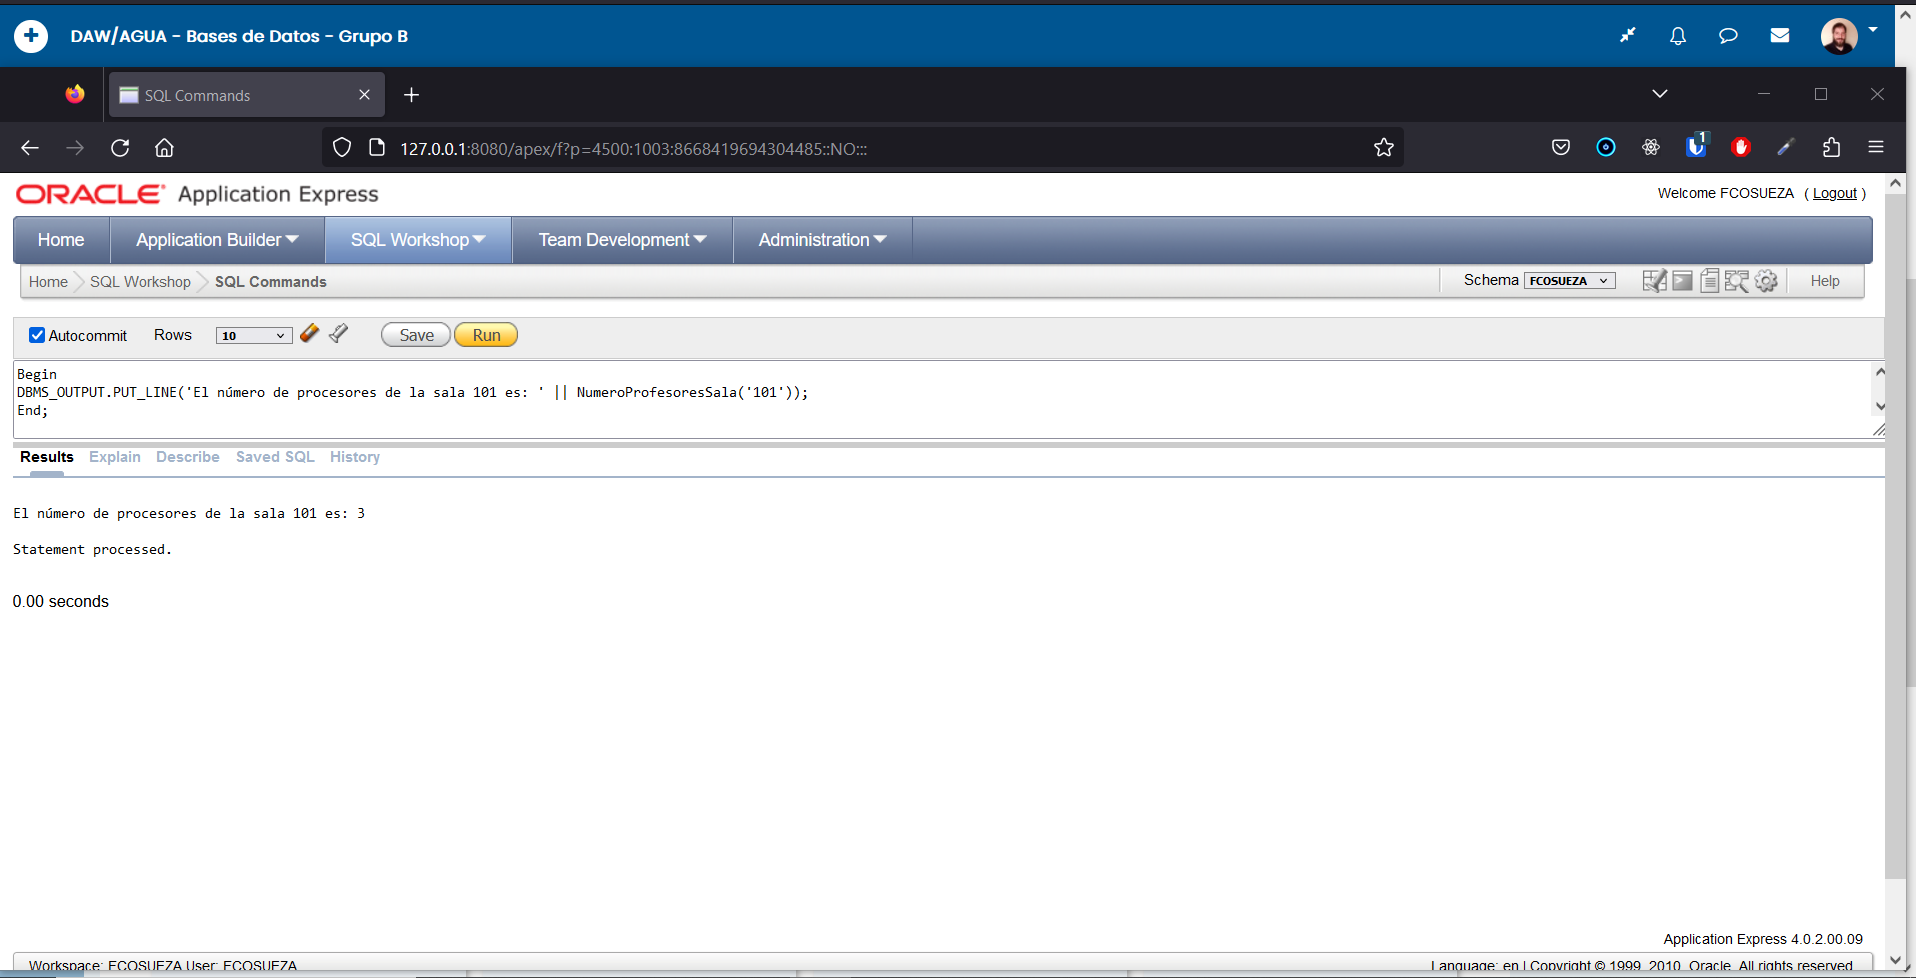
\includegraphics[scale=0.33]{funcion-ejecucion.png}
        \caption{Función NumeroProfesoresSala ejecutada en Oracle XE}
    \end{figure}

    \textbf{Disparador actulizaStock}:

    Por último, se ha creado un \textbf{disparador} o \textbf{trigger} para automatizar la actualización del stock de productos cada vez que se realiza una venta de estos.

    En primer lugar hemos usado la cláusula \textbf{BEFORE INSERT} en la definición del disparador porque debemos hacer una comprobación antes de actualizar la base de datos y permitir que se inserte la vente, que explicaremos en en los siguiente párrafos. También hemos usado la cláusula \textbf{FOR EACH ROW} ya que nos interesa que se actualice el stock de productos por cada venta realizada.

    Se han declarado varias variables, \textbf{stockTotal}, \textbf{stockMIN} y \textbf{nombreProducto} para almacenar el resultado de la consulta, usando un \textbf{INTO} dentro de está para almacenar la información en las variables.

    También se ha creado la variable \textbf{stockActualizado} para calcular el stock que habrá después de realizar la venta.

    Aquí es donde viene uno de los puntos clave. Si \textbf{intentamos vender más stock del que hay}, no debería permitirse realizar la operación \textbf{INSERT} ni realizar el \textbf{UPDATE} en la \textbf{tabla productos}. Esta segunda parte es fácil, ya que \textbf{controlamos} nosotros la sentencia de \textbf{actualización}, pero \textbf{no controlamos} la de \textbf{inserción}. Podríamos simplemente no actualizar el stock, pero entonces no tendríamos una \textbf{visión real} del stock que hay, por lo que lo ideal sería \textbf{no permitir esa venta}.

    \textbf{No se puede eliminar} al final del disparador la operación \textbf{INSERT}, aunque usemos la cláusula \textbf{AFTER INSERT}, ya que nos devolverá un \textbf{error} de que la \textbf{tabla esta mutando}. \textbf{Tampoco podemos usar} la función \textbf{ROLLBACK}, ya que no esta permitido su uso dentro de los triggers.

    Realmente, lo ideal sería hacer una comprobación en la operación de inserción, donde añadiríamos una condición dentro del \textbf{WHERE} para comprobar que hay suficiente stock para vender. Pero no tenemos control sobre este paso. Por lo que se ha optado por una \textbf{solución} no muy elegante, que es lanzar un error de aplicación si el número de stock que se quiere vender es mayor que el número de stock existente.

    Además, se comprobado si tras la venta, el número de stock esta por debajo del mínimo, lanzando un mensaje de aviso en caso afirmativo.

    En la siguiente imagen, tenemos una captura del disparador creado en Oracle XE.

    \begin{figure}[H]
        \centering
        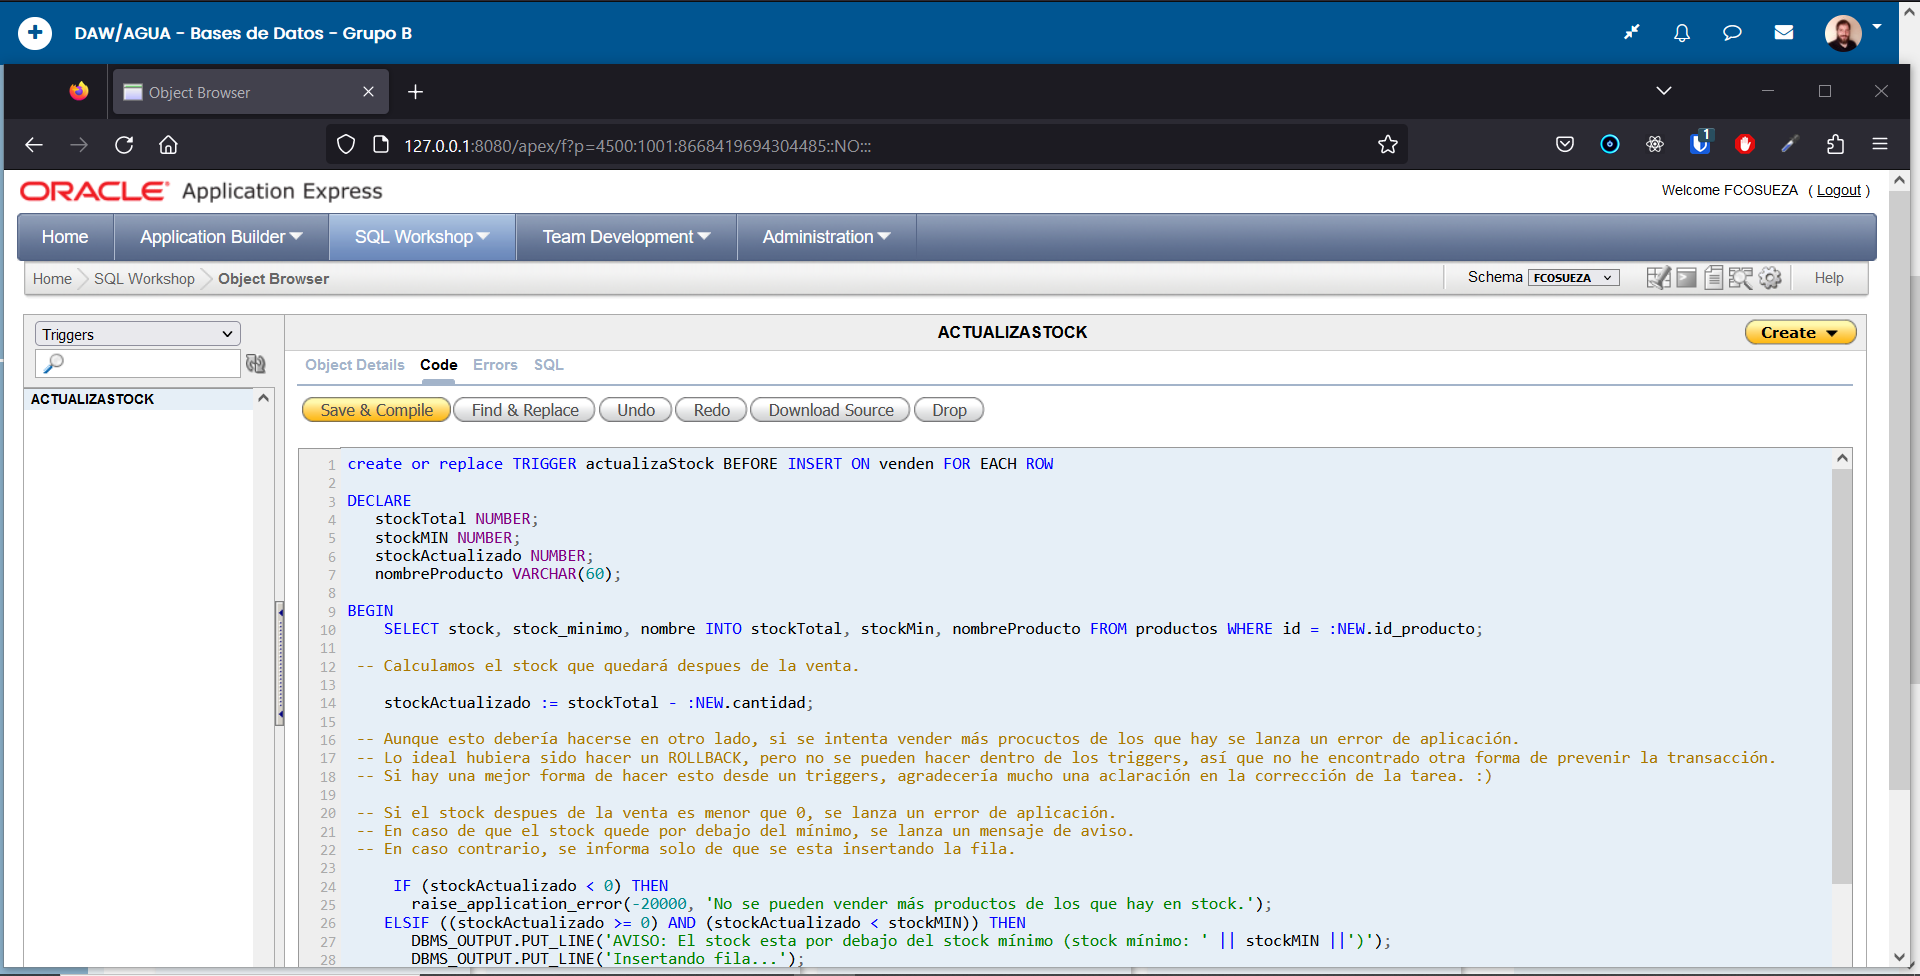
\includegraphics[scale=0.33]{trigger-1.png}
        \caption{Disparador creado en Oracle XE}
    \end{figure}

    Una vez creado, vamos a \textbf{comprobar que funciona correctamente}. Para ello en \textbf{primer lugar}, hemos comprobado la información que contiene la tabla productos antes de realizar la inserción en la tabla venden. Como vemos en la siguiente captura.

    \begin{figure}[H]
        \centering
        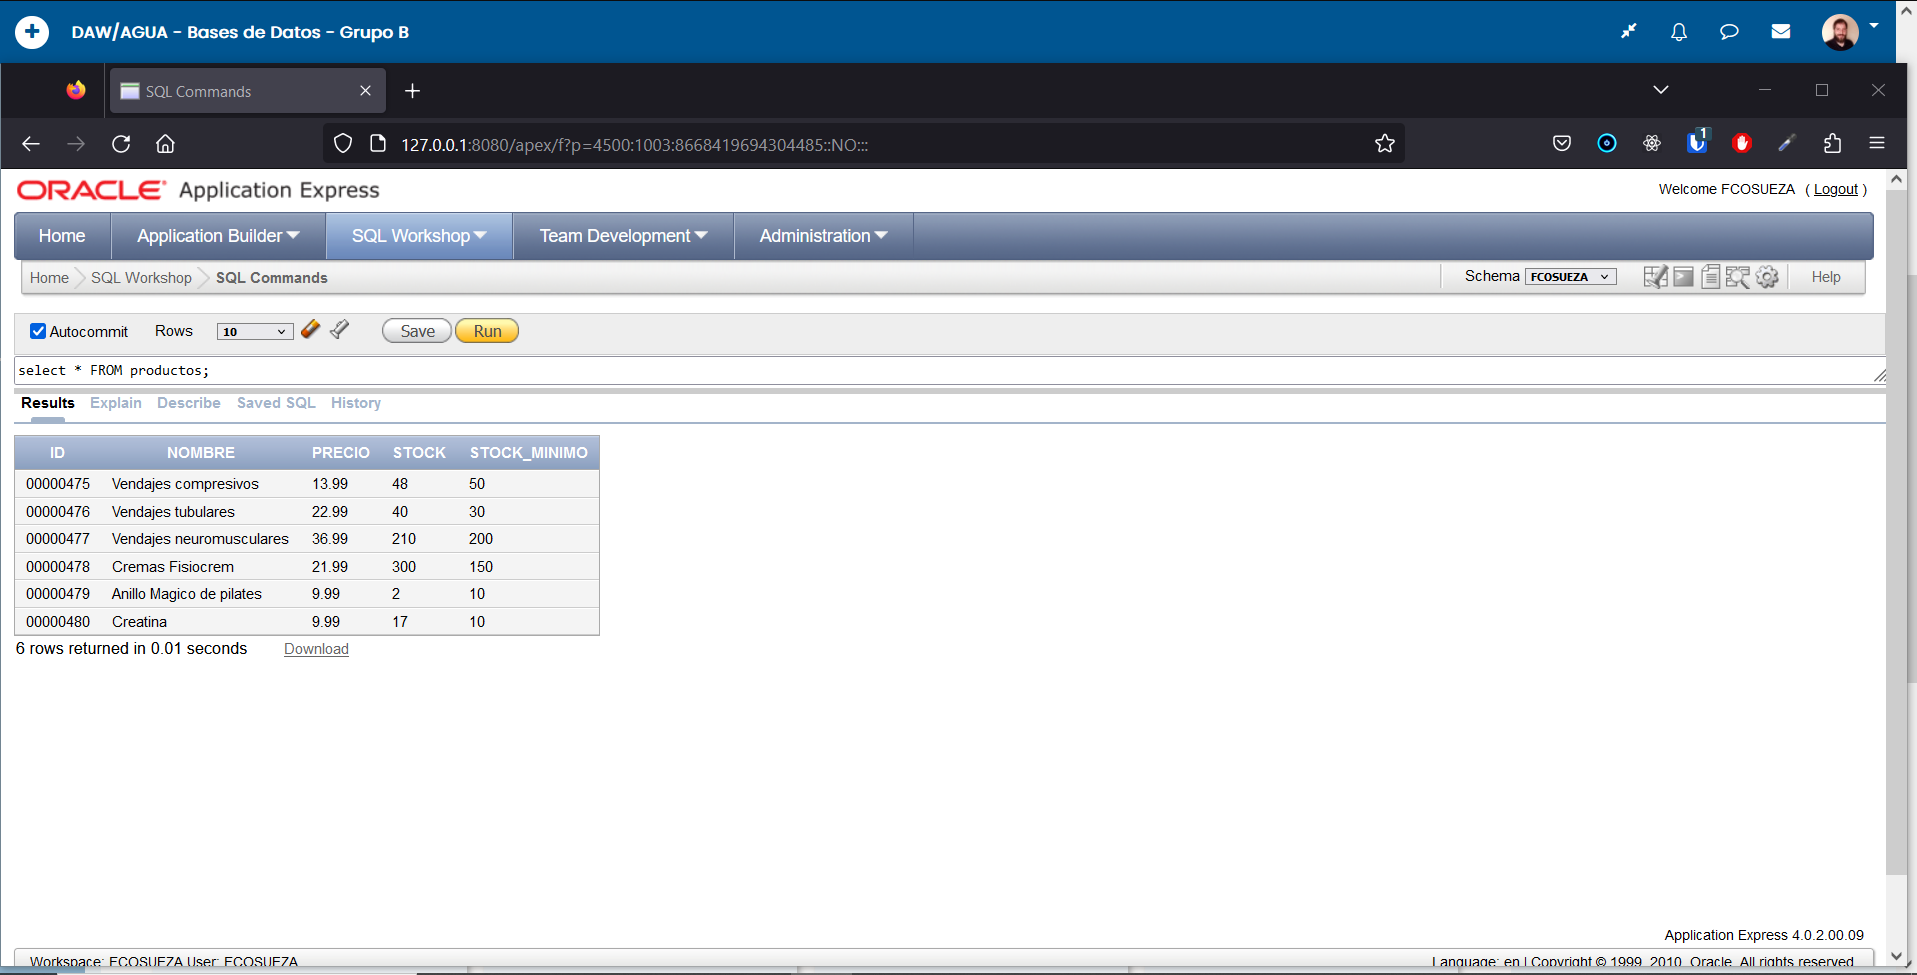
\includegraphics[scale=0.40]{trigger-2.png}
        \caption{Información tabla productos antes de la inserción}
    \end{figure}

    A continuación, hemos realizado una venta de  \textbf{5 Vendajes Tubulares}, como vemos en la siguiente captura, la cual se ha realizado correctamente.

        \begin{figure}[H]
        \centering
        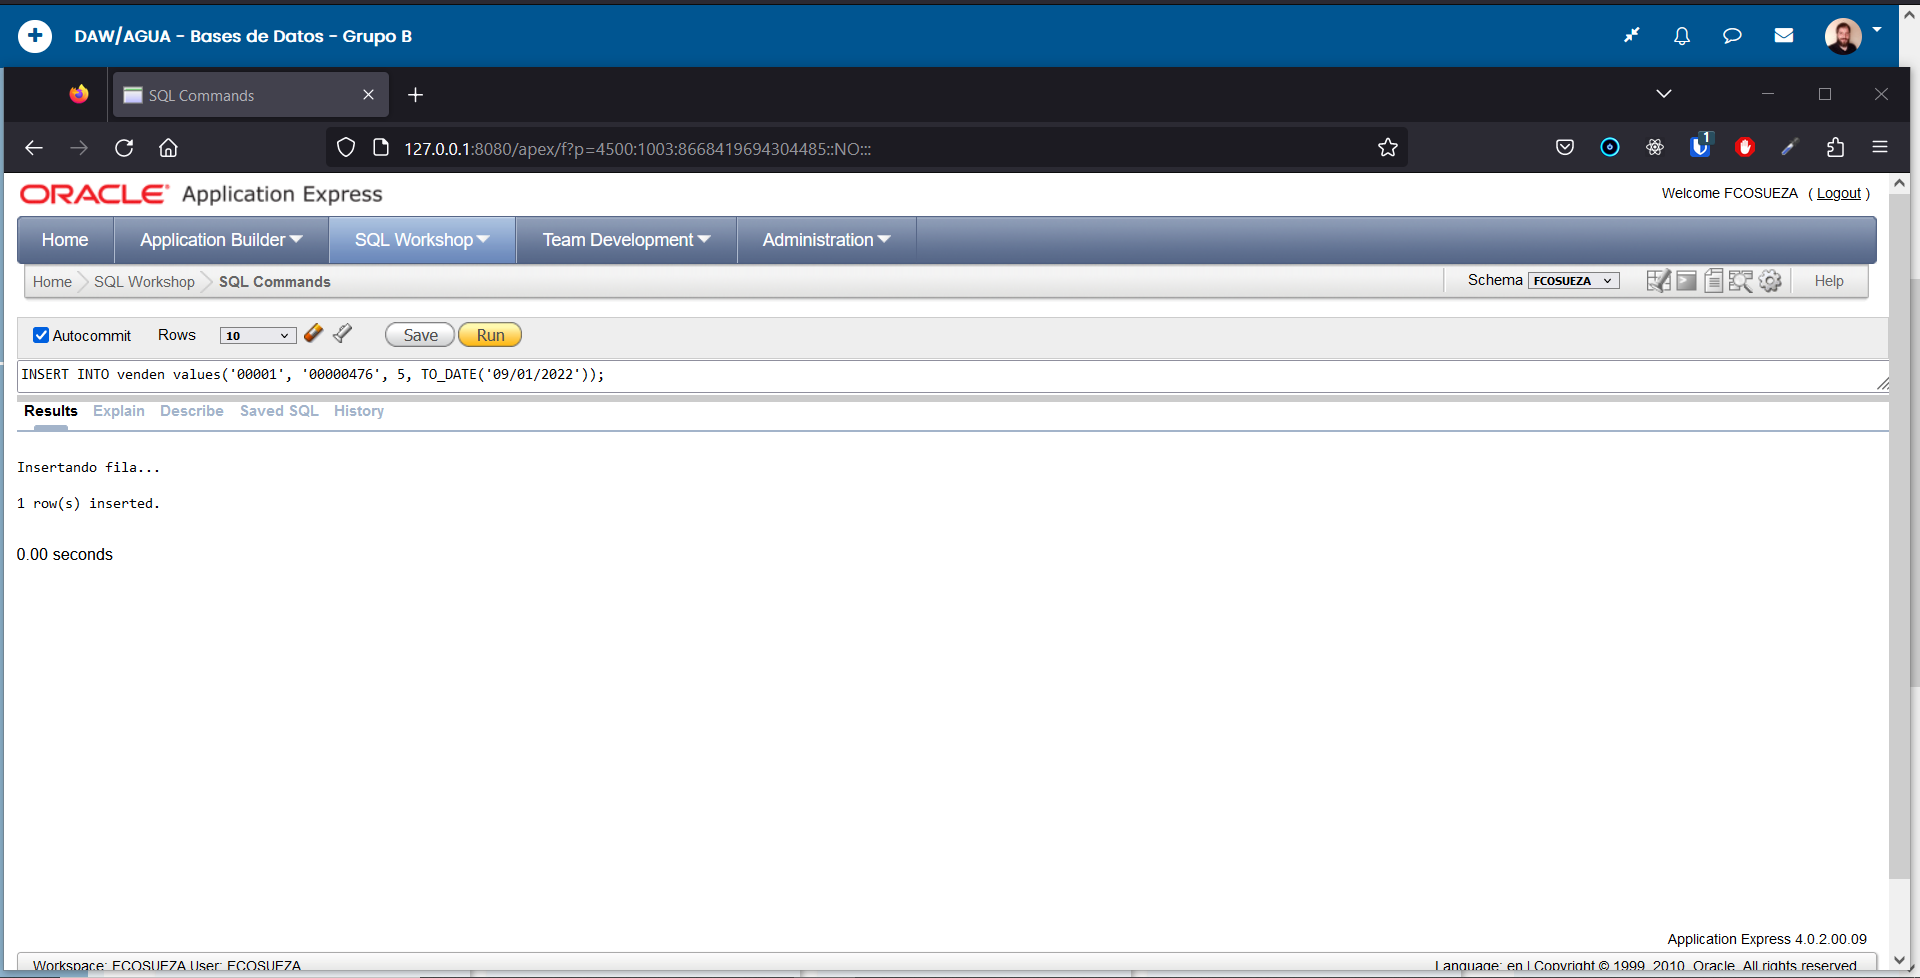
\includegraphics[scale=0.35]{trigger-3.png}
        \caption{Inserción en la tabla venden}
    \end{figure}

    Por último, hemos comprobado que la tabla productos se ha actualizado correctamente, es decir, que la fila de \textbf{Vendajes Tubulares} tiene un stock menor, en concreto, 5 unidades menor.

    Como hemos podido comprobar, y como se ve en la siguiente captura, la actualización se ha realizado correctamente.

        \begin{figure}[H]
        \centering
        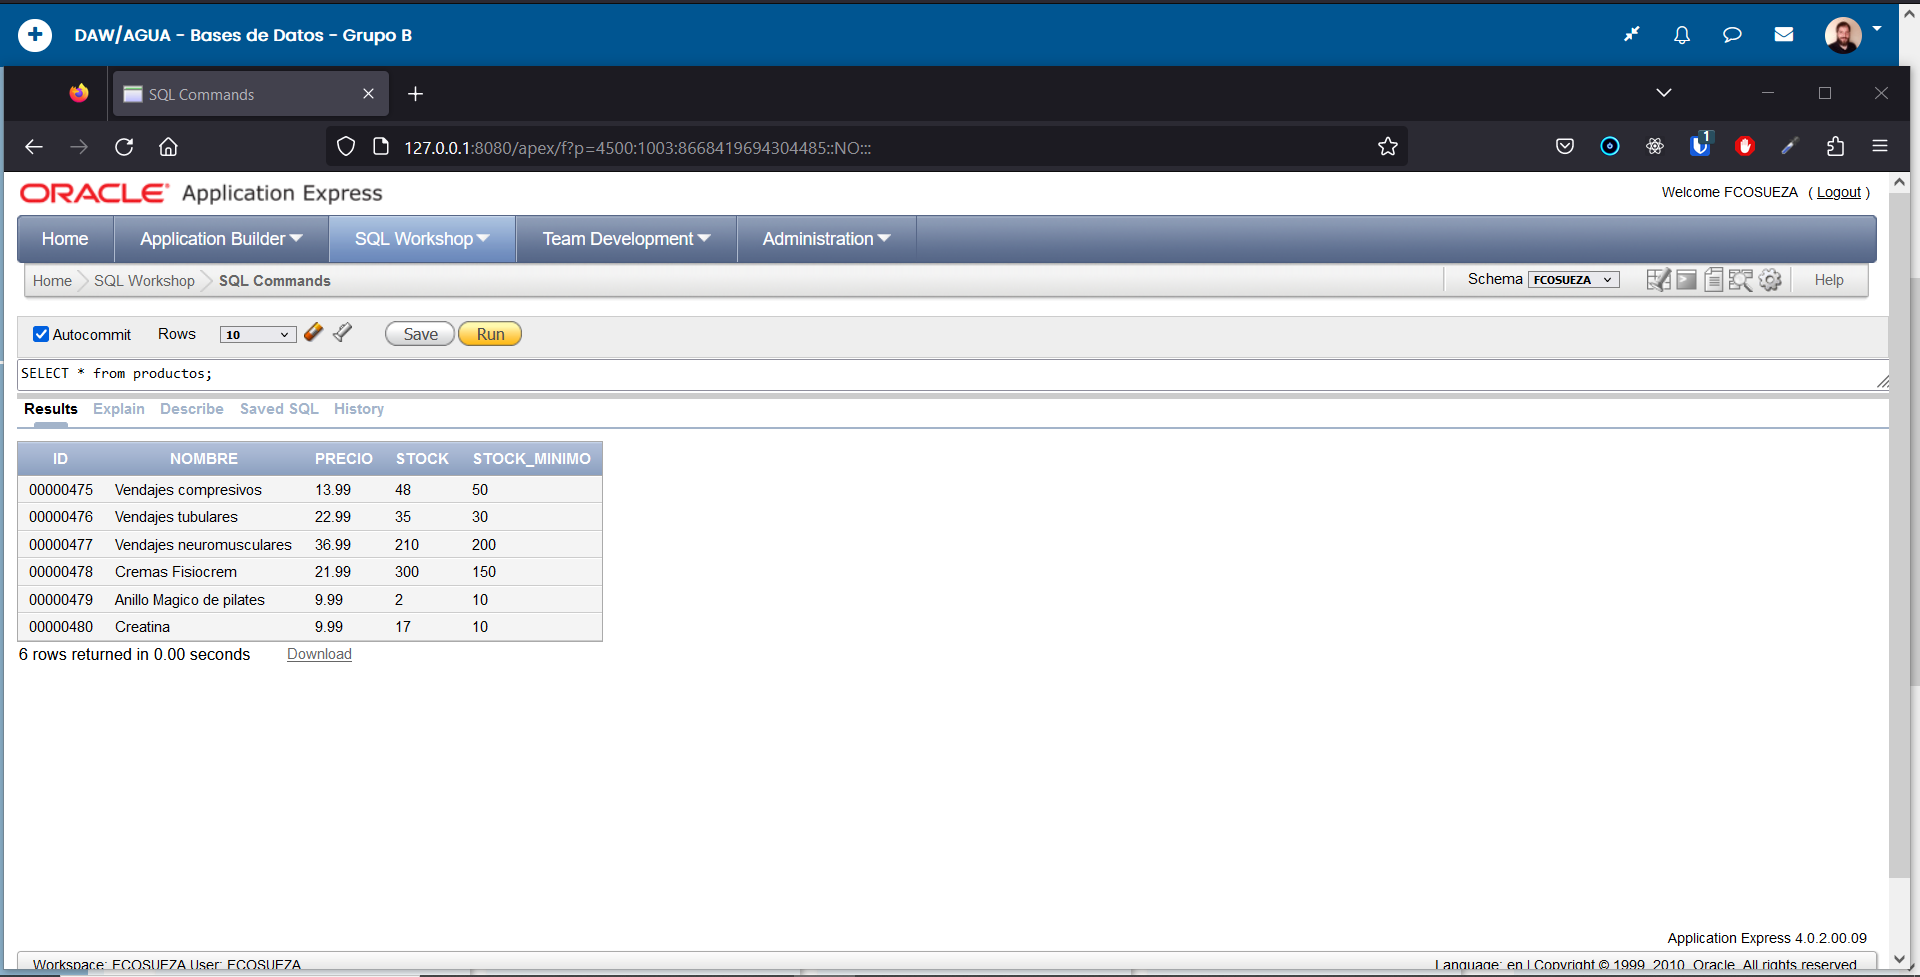
\includegraphics[scale=0.35]{trigger-4.png}
        \caption{Tabla productos actualizada}
    \end{figure}
\end{enumerate}

\section{Código Completo en PL/SQL}

\begin{figure}[H]
    \begin{tcolorbox}[sharp corners, colback=cyan!30, colframe=white!20]
\textbf{IMPORTANTE}:

El código no se muestra en orden, sino que se muestra por funciones adaptándolas
al espacio que hay libre en el documento, ya que no entra todo el código en una página,
aunque sea ha puesto pie de imagen en cada uno para indicar a que fragmento pertenece
este código. En el archivo que se adjunta viene todo el código en el orden adecuado.

También se han eliminado algunos comentarios en el código que aquí se muestra, y que
si están presentes en el archivos SQL que se adjunta, ya que sino los trozos de código
serían demasiado largos y no cabe en una misma página.
    \end{tcolorbox}
\end{figure}


\begin{figure}[H]
    \begin{tcolorbox}[sharp corners, colback=yellow!30, colframe=white!20]
        \tiny
        \begin{verbatim}
-- Función que devuelve el número de profesores de pilates diferentes que imparten clases en una sala dada.

create or replace FUNCTION NumeroProfesoresSala(vCodigoSala VARCHAR2) RETURN NUMBER IS nProfesores NUMBER;

BEGIN
SELECT count(DISTINCT numero_trabajador_pilates) INTO nProfesores
FROM imparte
WHERE codigo_sala = vCodigoSala;

RETURN nProfesores;

END NumeroProfesoresSala;
        \end{verbatim}
    \end{tcolorbox}
    \caption{Código de la función NumeroProfesoresSala}
\end{figure}


\begin{figure}[H]
    \begin{tcolorbox}[sharp corners, colback=yellow!30, colframe=white!20]
        \tiny
        \begin{verbatim}

-- Procedimiento para calcular el número de clientes que han tenido con un fisioterapeuta dado.

create or replace PROCEDURE NumeroCLientesFisio(pNumeroFisio VARCHAR2)
AS
CURSOR clientesFisio IS
SELECT cli.nombre, cli.apellidos, cli.dni, cli.telefono, ci.fecha_hora, ci.precio
FROM cita ci, cliente cli
WHERE ci.numero_fisio = pNumeroFisio AND ci.dni_cliente = cli.dni;

invalid_param EXCEPTION;
PRAGMA exception_init(invalid_param, -404);

rowClientes clientesFisio%ROWTYPE;

BEGIN

if (LENGTH(pNumeroFisio) <> 5) THEN
RAISE invalid_param;
END IF;

open clientesFisio;
fetch clientesFisio INTO rowClientes;

DBMS_OUTPUT.PUT_LINE('El fisio con número: ' || pNumeroFisio || ' ha tenido cita con los siguientes clientes: ');
DBMS_OUTPUT.PUT_LINE('----------------------------------------------------------------------------------------------');
DBMS_OUTPUT.PUT_LINE('CLIENTES                        DNI           TELEFONO        FECHA                PRECIO     ');
DBMS_OUTPUT.PUT_LINE('----------------------------------------------------------------------------------------------');

WHILE clientesFisio%FOUND LOOP
    DBMS_OUTPUT.PUT_LINE(
        RPAD(rowCLientes.nombre, 10) || RPAD(rowCLientes.apellidos, 22) ||
        RPAD(rowClientes.dni, 14) || RPAD(rowClientes.telefono, 16) ||
        RPAD(TO_CHAR(rowClientes.fecha_hora, 'DD-MM-YYYY HH:MI'), 21) || rowClientes.precio|| '€' );

fetch clientesFisio INTO rowCLientes;
END LOOP;

CLOSE clientesFisio;

EXCEPTION
    WHEN invalid_param THEN
        DBMS_OUTPUT.PUT_LINE('El identificador del fisioterapeuta debe ser una cadena de 5 caracteres, ejemplo: 00001');

END NumeroClientesFisio;
        \end{verbatim}
    \end{tcolorbox}
    \caption{Código del Procedimiento NumeroClientesFisio}
\end{figure}

\begin{figure}[H]
    \begin{tcolorbox}[sharp corners, colback=yellow!30, colframe=white!20]
        \tiny
        \begin{verbatim}

create or replace TRIGGER actualizaStock BEFORE INSERT ON venden FOR EACH ROW

DECLARE
stockTotal NUMBER;
stockMIN NUMBER;
stockActualizado NUMBER;
nombreProducto VARCHAR(60);

BEGIN
SELECT stock, stock_minimo, nombre INTO stockTotal, stockMin, nombreProducto
FROM productos
WHERE id = :NEW.id_producto;

-- Calculamos el stock que quedará despues de la venta.

stockActualizado := stockTotal - :NEW.cantidad;


IF (stockActualizado < 0) THEN
raise_application_error(-20000, 'No se pueden vender más productos de los que hay en stock.');
ELSIF ((stockActualizado >= 0) AND (stockActualizado < stockMIN)) THEN
DBMS_OUTPUT.PUT_LINE('AVISO: El stock esta por debajo del stock mínimo (stock mínimo: ' || stockMIN ||')');
DBMS_OUTPUT.PUT_LINE('Insertando fila...');
ELSE
DBMS_OUTPUT.PUT_LINE('Insertando fila...');
END IF;

-- Se actualiza la tabla productos con la nueva cantidad del producto vendido.

UPDATE productos SET stock = stockActualizado WHERE id = :NEW.id_producto;

END actualizaStock;
        \end{verbatim}
    \end{tcolorbox}
    \caption{Código del disparador}
\end{figure}

\begin{figure}[H]
    \begin{tcolorbox}[sharp corners, colback=yellow!30, colframe=white!20]
        \tiny
        \begin{verbatim}
create or replace PROCEDURE CitasFisio(pDNI VARCHAR2)
AS
CURSOR cCitas IS
SELECT cli.dni, cli.nombre, cli.apellidos, cli.descuento, ci.precio
FROM cliente cli, cita ci
WHERE ci.dni_cliente = pDNI AND ci.dni_cliente = cli.dni;

-- Creamos una excepción por si el DNI no se introduce con la longitud adecuada

invalid_param EXCEPTION;
PRAGMA exception_init(invalid_param, -404);

cCitasRow cCitas%ROWTYPE;
precioTotal FLOAT := 0.0;
descuento FLOAT;

BEGIN

-- Si el DNI introducido no tiene el tamaño adecuado lanzamos una excepción.

if (LENGTH(pDNI) <> 9) THEN
RAISE invalid_param;
END IF;

OPEN cCitas;
FETCH cCitas INTO cCitasRow;

WHILE cCitas%FOUND LOOP
precioTotal := precioTotal + cCitasRow.precio;
FETCH cCitas INTO cCitasRow;
END LOOP;

-- Calculamos el descuento a aplicar

descuento := (cCitasRow.descuento * precioTotal) / 100;


DBMS_OUTPUT.PUT_LINE('El DNI del clientes es: ' || pDNI);
DBMS_OUTPUT.PUT_LINE('El nombre del clientes es: ' || cCitasRow.nombre);
DBMS_OUTPUT.PUT_LINE('Los apellidos del cliente son: ' || cCitasRow.apellidos);
DBMS_OUTPUT.PUT_LINE('El numero total de citas es: ' || cCitas%ROWCOUNT);
DBMS_OUTPUT.PUT_LINE('El precio total de las citas es: '  || precioTotal);
DBMS_OUTPUT.PUT_LINE('El descuento es: ' || cCitasRow.descuento || '%');
DBMS_OUTPUT.PUT_LINE('El precio final es: ' || (precioTotal - descuento));

CLOSE cCitas;

-- Procesamos la excepción invalid_param si se ha lanzado y mostramos un mensaje de ayuda

EXCEPTION
WHEN invalid_param THEN
DBMS_OUTPUT.PUT_LINE('El DNI del cliente debe ser una cadena de 9 caracteres, ejemplo: 75192847W');

        \end{verbatim}
    \end{tcolorbox}
    \caption{Código del procedimiento CitasFisio}
\end{figure}
% Bibliography

%\newpage
%\bibliography{citas}
%\bibliographystyle{unsrt}

\end{document}